\documentclass[a4paper, 12pt]{article}

% --- Пакеты ---
\usepackage[T2A]{fontenc}
\usepackage[utf8]{inputenc}
\usepackage[russian]{babel}
\usepackage{amsmath}
\usepackage{graphicx}
\usepackage{float}
\usepackage[left=2.5cm, right=1.5cm, top=2cm, bottom=2cm]{geometry}
\usepackage[unicode]{hyperref}

% <<< ИЗМЕНЕНИЕ: Убираем пакет tcolorbox
% \usepackage[skins]{tcolorbox}
% \newtcolorbox{mybox}{...}

% <<< ИЗМЕНЕНИЕ: Создаем новое, более простое окружение для выводов
\newenvironment{conclusion}
  {\begin{quote}\noindent\textbf{Выводы: }\itshape}
  {\end{quote}}

\begin{document}

% ===================================================================
% ЭКСПЕРИМЕНТ 1 (ПОЛНОСТЬЮ ОБНОВЛЕННАЯ ВЕРСИЯ С ДВУМЯ ГРАФИКАМИ)
% ===================================================================
\section{Сравнение метрик для разных обучающих выборок}

\subsection{Описание эксперимента}
Данный эксперимент сравнивает 3 метрики при предсказании на 10 шагов вперед: RMSE, доля непрогнозируемых точек, MAPE для разных обучающих выборок.

Были посчитаны метрики для обучающей выборки, состоящей из 10000 точек ряда с $\sigma=10, r=28, b=8/3$, для которого мы предсказываем и переменным количеством точек ряда с другим значением $r$. Были подсчитаны метрики для обучающей выборки из переменного количества точек базового ряда с $\sigma=10, r=28, b=8/3$.

\subsection{Результаты}

\begin{figure}[H]
    \begin{minipage}[c]{0.3\textwidth} 
        Для наглядной оценки выигрыша или проигрыша от добавления данных из "соседних" рядов, метрики RMSE и MAPE были нормированы на соответствующие значения для "чистого" ряда с $r=28$.
        \vspace{\baselineskip}
        
        Значение 1.0 (пунктирная линия) соответствует базовому случаю. Значения ниже 1.0 означают улучшение, выше — ухудшение.
        \vspace{\baselineskip}
        
        На этом графике показаны наиболее удачные случаи, где для добавленного ряда с $r=27.9$ и $r=27.99$ получаются результаты, сравнимые с базовым рядом.
    \end{minipage}
    \hfill 
    \begin{minipage}[c]{0.68\textwidth} 
        \centering
        % ПРОВЕРЬТЕ ПУТЬ К ФАЙЛУ
        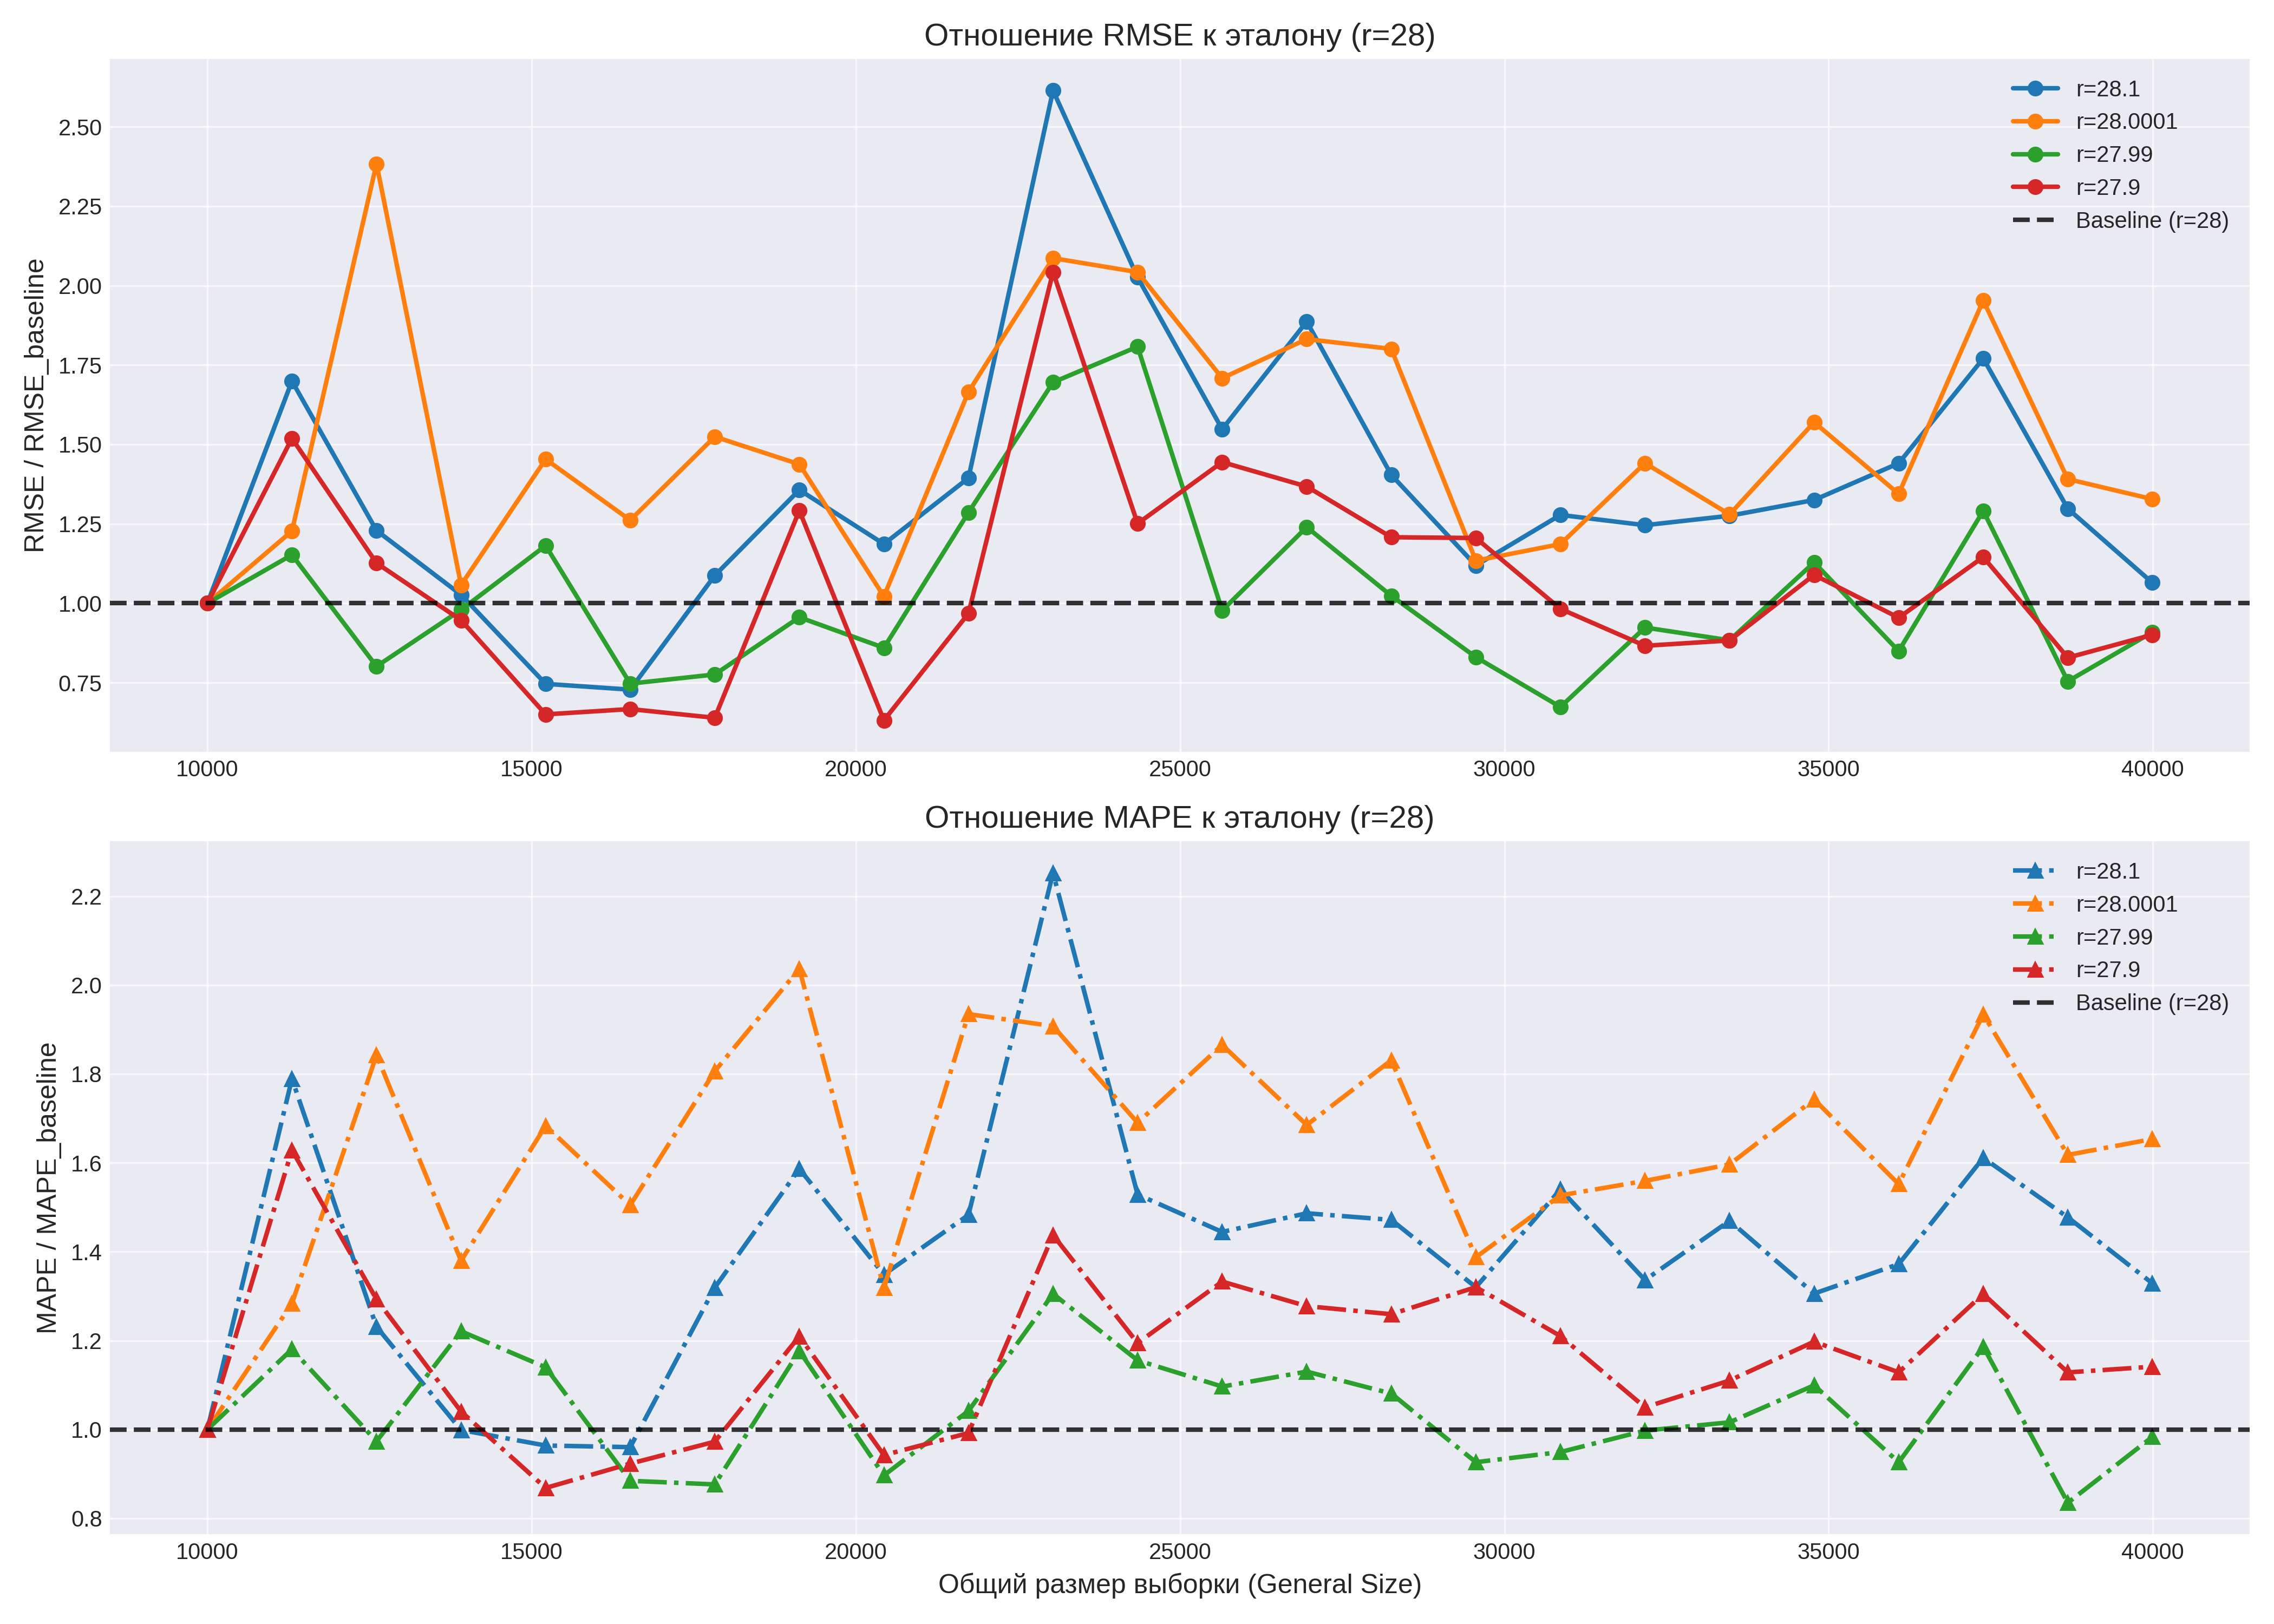
\includegraphics[width=\textwidth]{./Size_experiment/metrics_ratio_vs_general_size.png}
        \caption{Зависимость относительных метрик для удачных экспериментов.}
        \label{fig:ratio_exp_best}
    \end{minipage}
\end{figure}

\begin{figure}[H]
    \begin{minipage}[c]{0.3\textwidth} 
        На этом графике аналогичным образом показаны менее удачные расширения обучающих выборок (с $r=28.01, r=30, r=38, r=27$).
        \vspace{\baselineskip}
        
        Видно, что они не дают выигрыша по всем трем метрикам одновременно, но могут дать выигрыш по количеству непрогнозируемых точек.
    \end{minipage}
    \hfill
    \begin{minipage}[c]{0.68\textwidth}
        \centering
        % ПРОВЕРЬТЕ ПУТЬ К ФАЙЛУ
        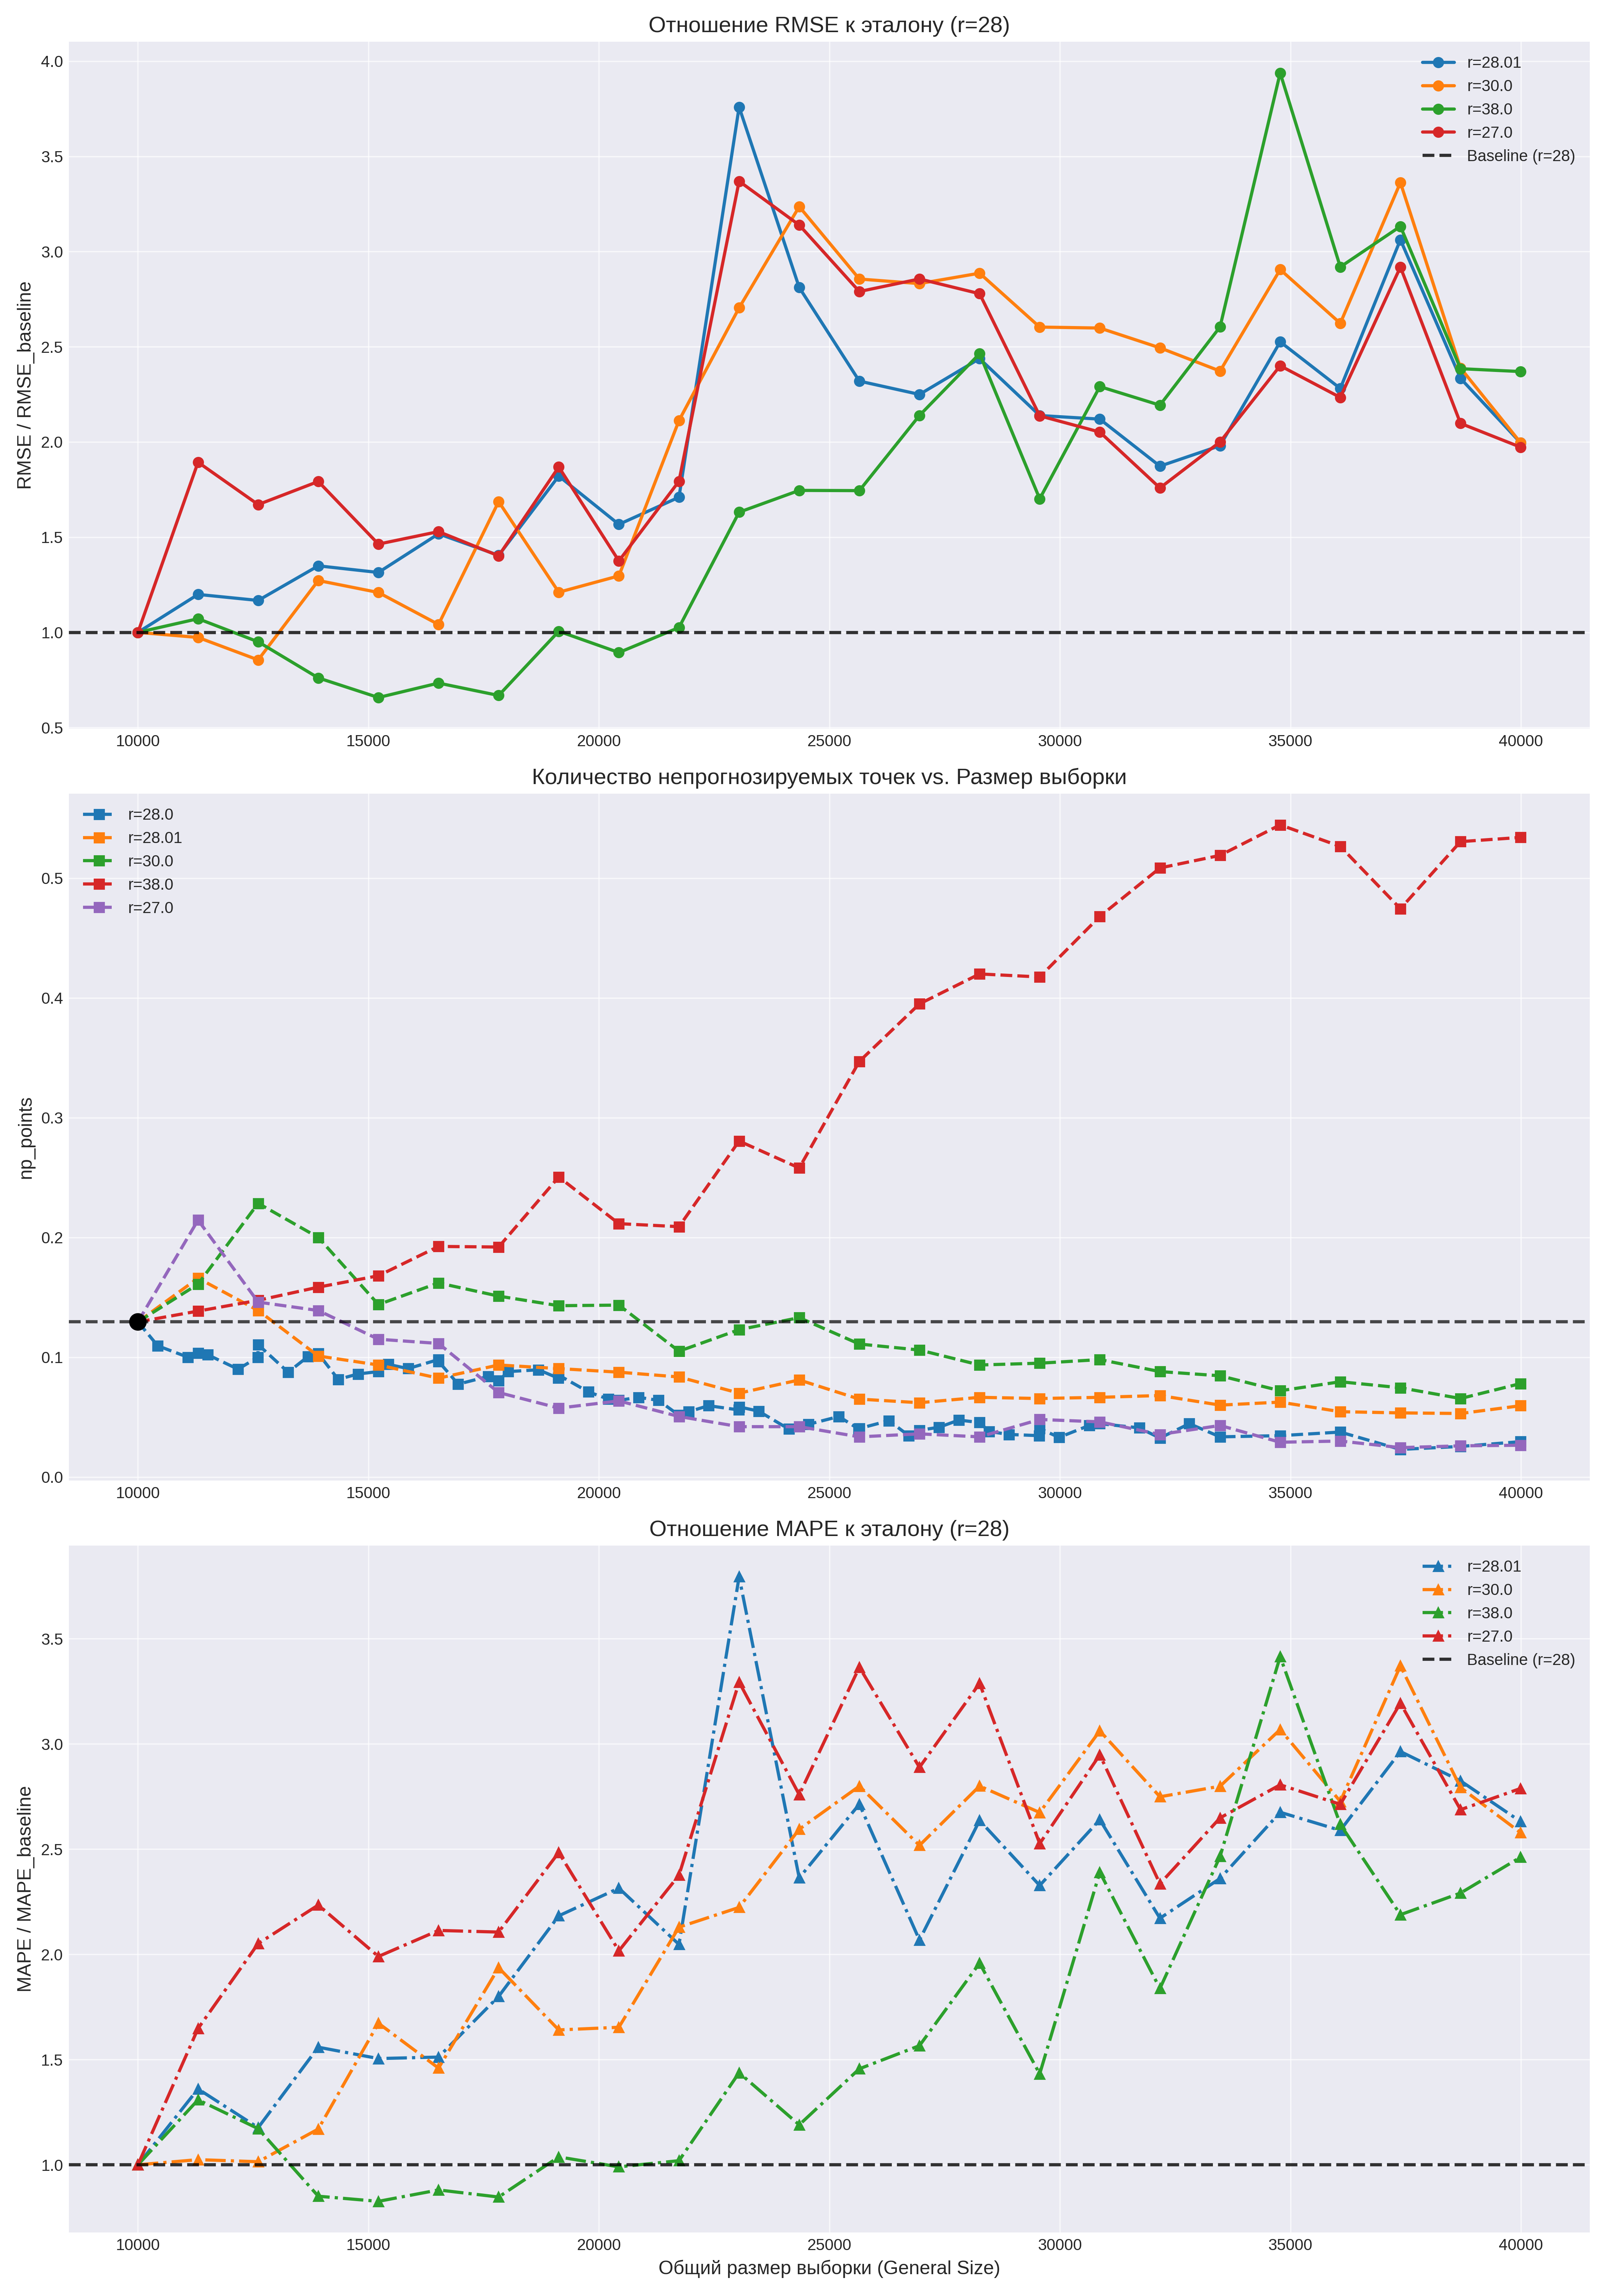
\includegraphics[width=\textwidth]{./Size_experiment/metrics_comparison_with_ratios_unlucky.png}
        \caption{Зависимость относительных метрик для менее удачных экспериментов.}
        \label{fig:ratio_exp_unlucky}
    \end{minipage}
\end{figure}


\begin{conclusion}
    Для добавленного ряда с $r=27.9$ и $r=27.99$ получаются результаты сравнимые по всем метрикам с выборкой только на основе базового ряда.
    
    Менее удачные расширения обучающих выборок (с $r=28.01, r=30, r=38, r=27$) не дают выигрыш по всем трем метрикам, но могут дать выигрыш по количеству непрогнозируемых точек или метрикам качества предсказания.
    
    Почему предсказание с $r=28.0001$ хуже чем с $r=28.1$ меня вгоняет в тупик.
\end{conclusion}

% ===================================================================
% КОНЕЦ ПЕРВОГО ЭКСПЕРИМЕНТА
% ===================================================================
% ===================================================================
% ВТОРОЙ ЭКСПЕРИМЕНТ
% ===================================================================
\newpage 

\section{Эксперимент по изменению параметров выборки}

\subsection{Описание эксперимента}
Данный эксперимент сравнивает 3 метрики при предсказании на 10 шагов вперед: RMSE, доля непрогнозируемых точек, MAPE для разных обучающих выборок.

Сравнивались три сценария:
\begin{enumerate}
    \item Обучающая выборка из 5000 точек базового ряда ($\sigma=10, r=28, b=8/3$)
     и 5000 точек ряда с другим значением $r$.
    \item Оптимальная выборка из 10000 точек базового ряда ($r=28$).
    \item Базовая выборка из 5000 точек базового ряда ($r=28$).
\end{enumerate}

\subsection{Результаты}

\begin{figure}[H]
    \begin{minipage}[c]{0.3\textwidth} 
        Из результатов видно, что в небольшой окрестности вокруг $r$ при добавлении 
        ряда с другим параметром наблюдается улучшение всех метрик относительно
         обучающей выборки из 5000 точек основного ряда.
        \vspace{\baselineskip}
        
        Однако метрики всегда получаются хуже по сравнению с обучающей выборкой из 10000 точек.
    \end{minipage}
    \hfill 
    \begin{minipage}[c]{0.68\textwidth} 
        \centering
        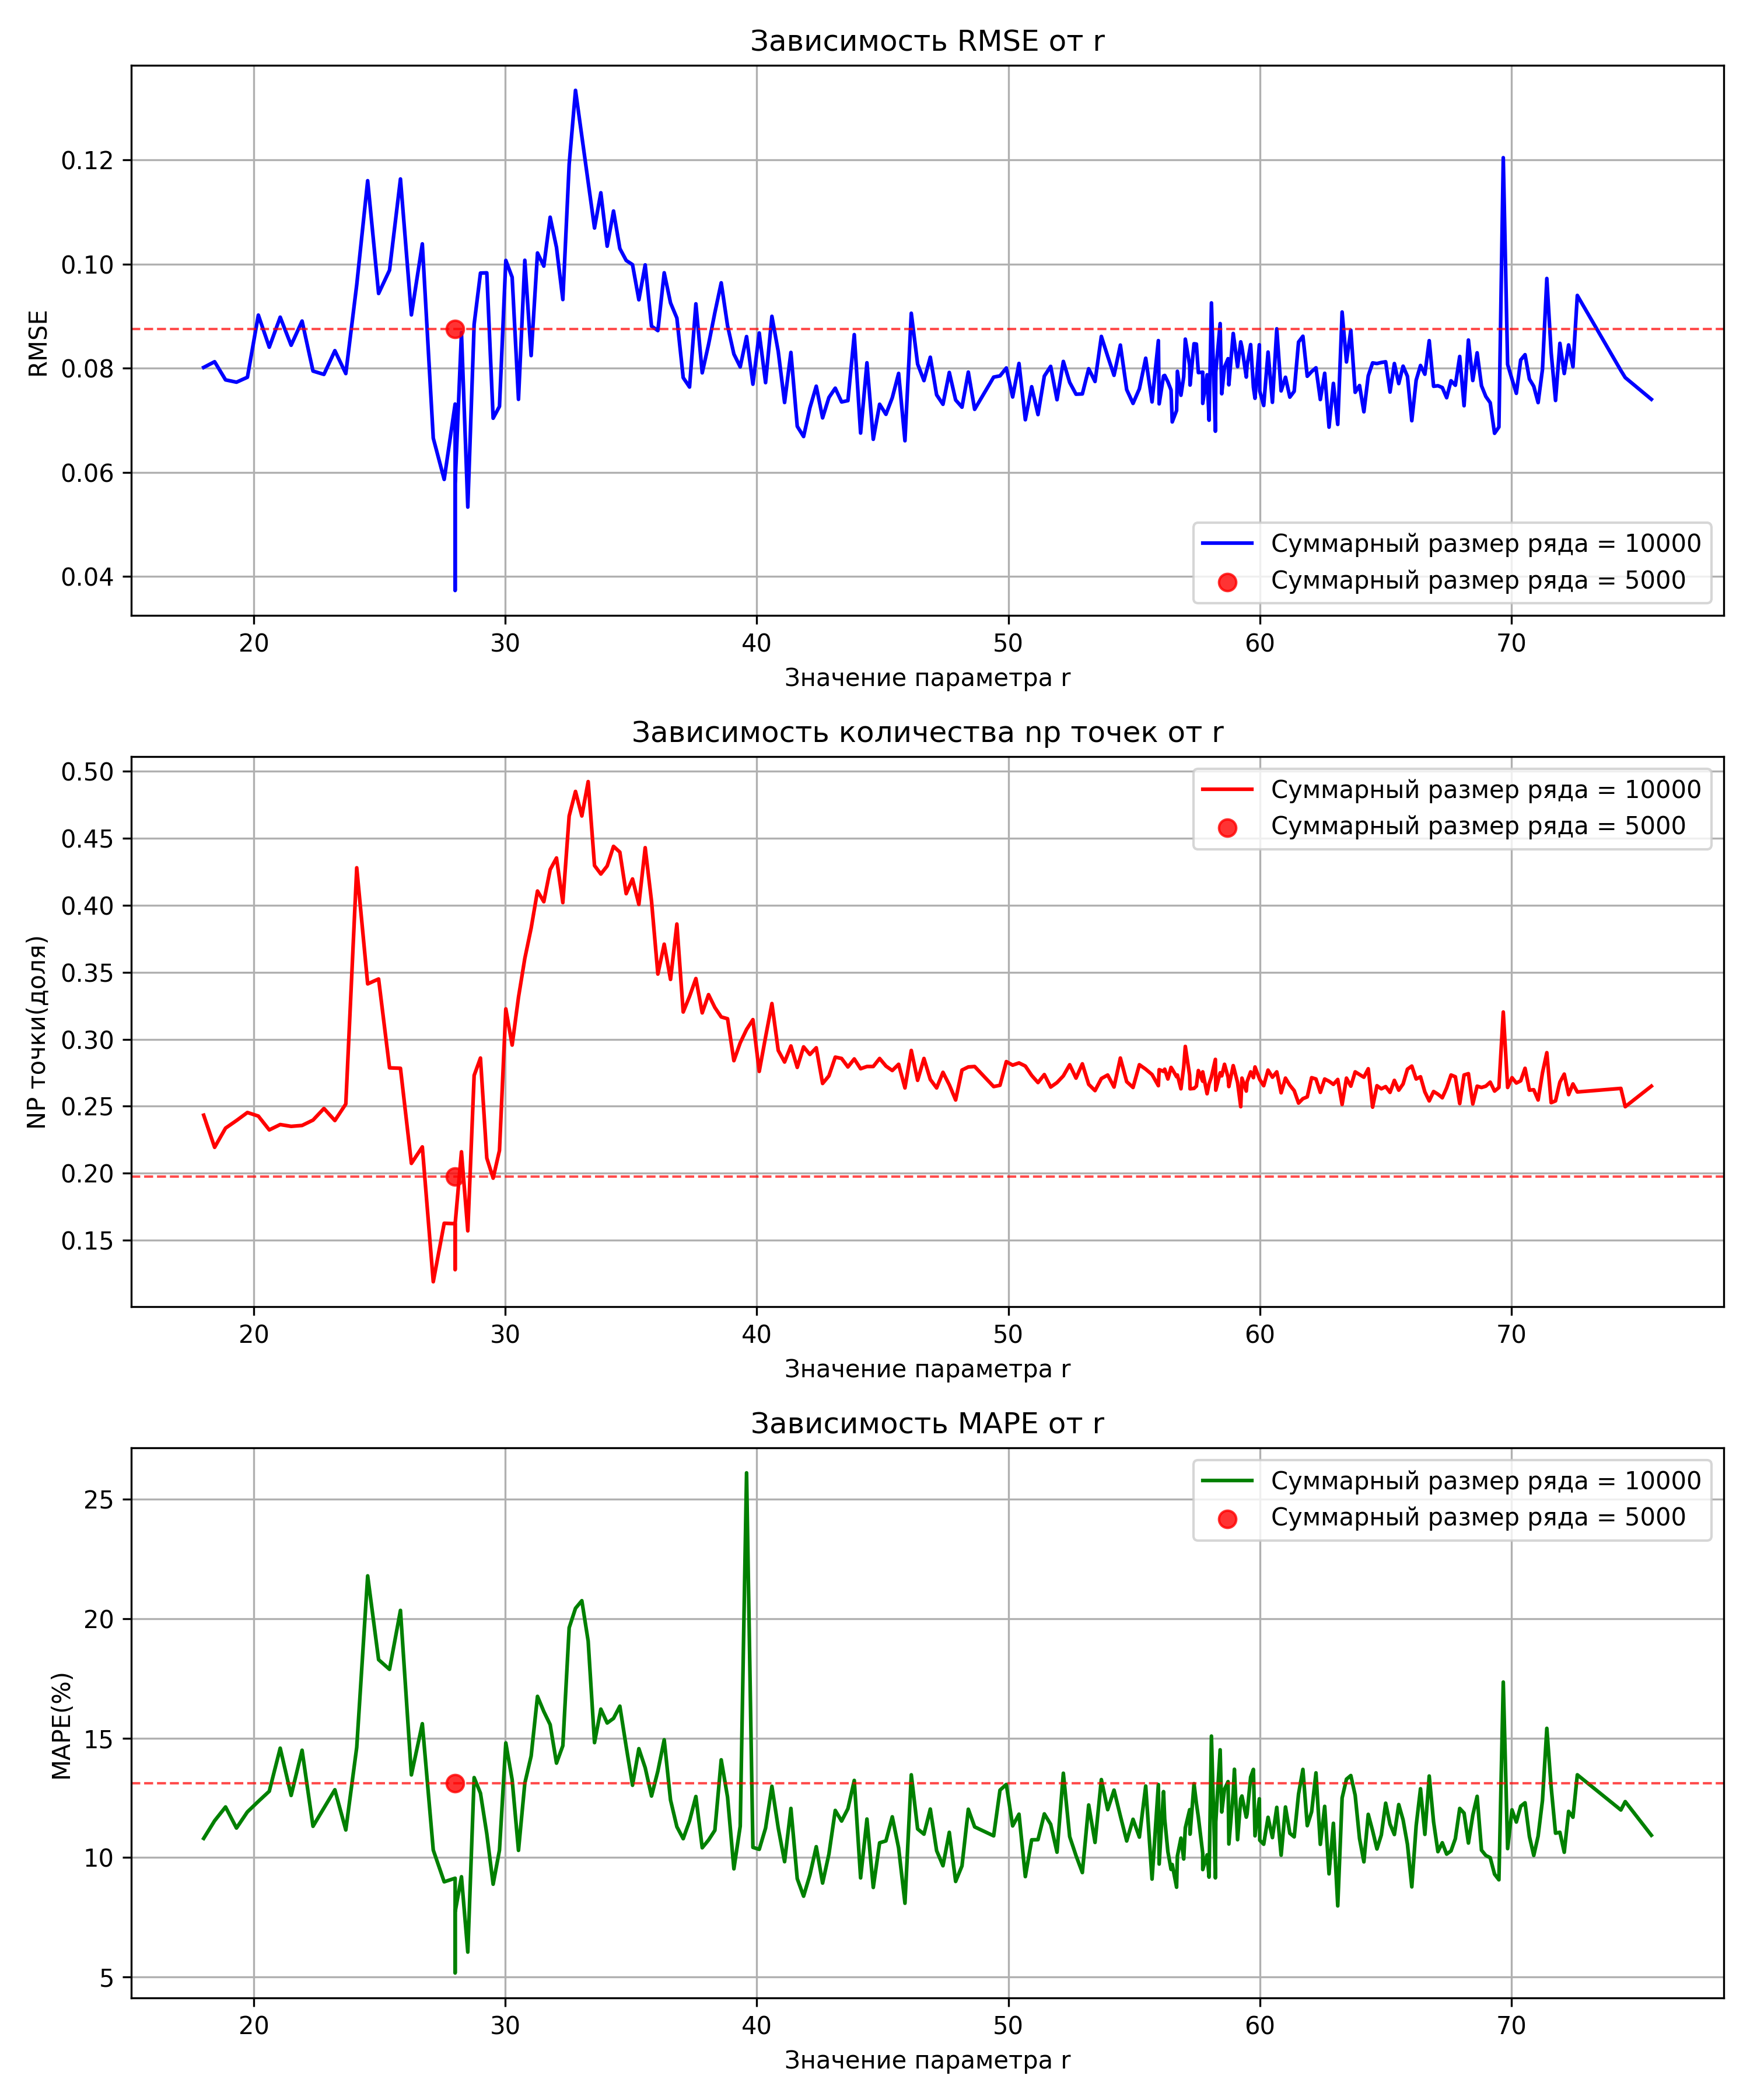
\includegraphics[width=\textwidth]{./deviations/Разные_r.png}
        \caption{Зависимость метрик от параметра $r$ в добавленной выборке (5000+5000 точек).}
        \label{fig:diff_r_exp}
    \end{minipage}
\end{figure}

% <<< ИЗМЕНЕНИЕ: Заменяем mybox на conclusion
\begin{conclusion}
    Согласно этому эксперименту центральная идея задачи выполняется. 
    Добавление рядов из небольшой окрестности расширяет выборку, 
    позволяя лучше предсказывать, чем без нее. Это происходит даже 
    несмотря на то, что мы создаем две близкие друг к другу выборки 
    на одинаковых участках: то есть мы берем в добавленном ряду не точки 
    с 5001 по 10000, а точки с 1 по 5000, что покрывает примерно тот же
     кусок ряда что и исходный ряд на первые 5 тысяч точек.
\end{conclusion}

% ===================================================================
% ТРЕТИЙ ЭКСПЕРИМЕНТ
% ===================================================================
\newpage

\section{Эксперимент 3: Вычисление DTW}

\subsection{Описание эксперимента}
ТЕКСТ.

\subsection{Результаты}

\begin{figure}[H]
    \begin{minipage}[c]{0.3\textwidth} 
        Результаты вычислений DTW:
        \vspace{\baselineskip}
        
        { 
        \setlength{\tabcolsep}{3pt} 
        \begin{tabular}{lr}
        \hline
        \textbf{$r$} & \textbf{DTW} \\ 
        \hline
        28.0001 & 16386.42 \\
        27.99   & 16994.62 \\
        28.01   & 18952.64 \\
        28.1    & 17823.66 \\
        27.9    & 19479.54 \\
        30      & 20504.81 \\
        \hline
        \end{tabular}
        } 
        
    \end{minipage}
    \hfill 
    \begin{minipage}[c]{0.68\textwidth} 
        \centering
        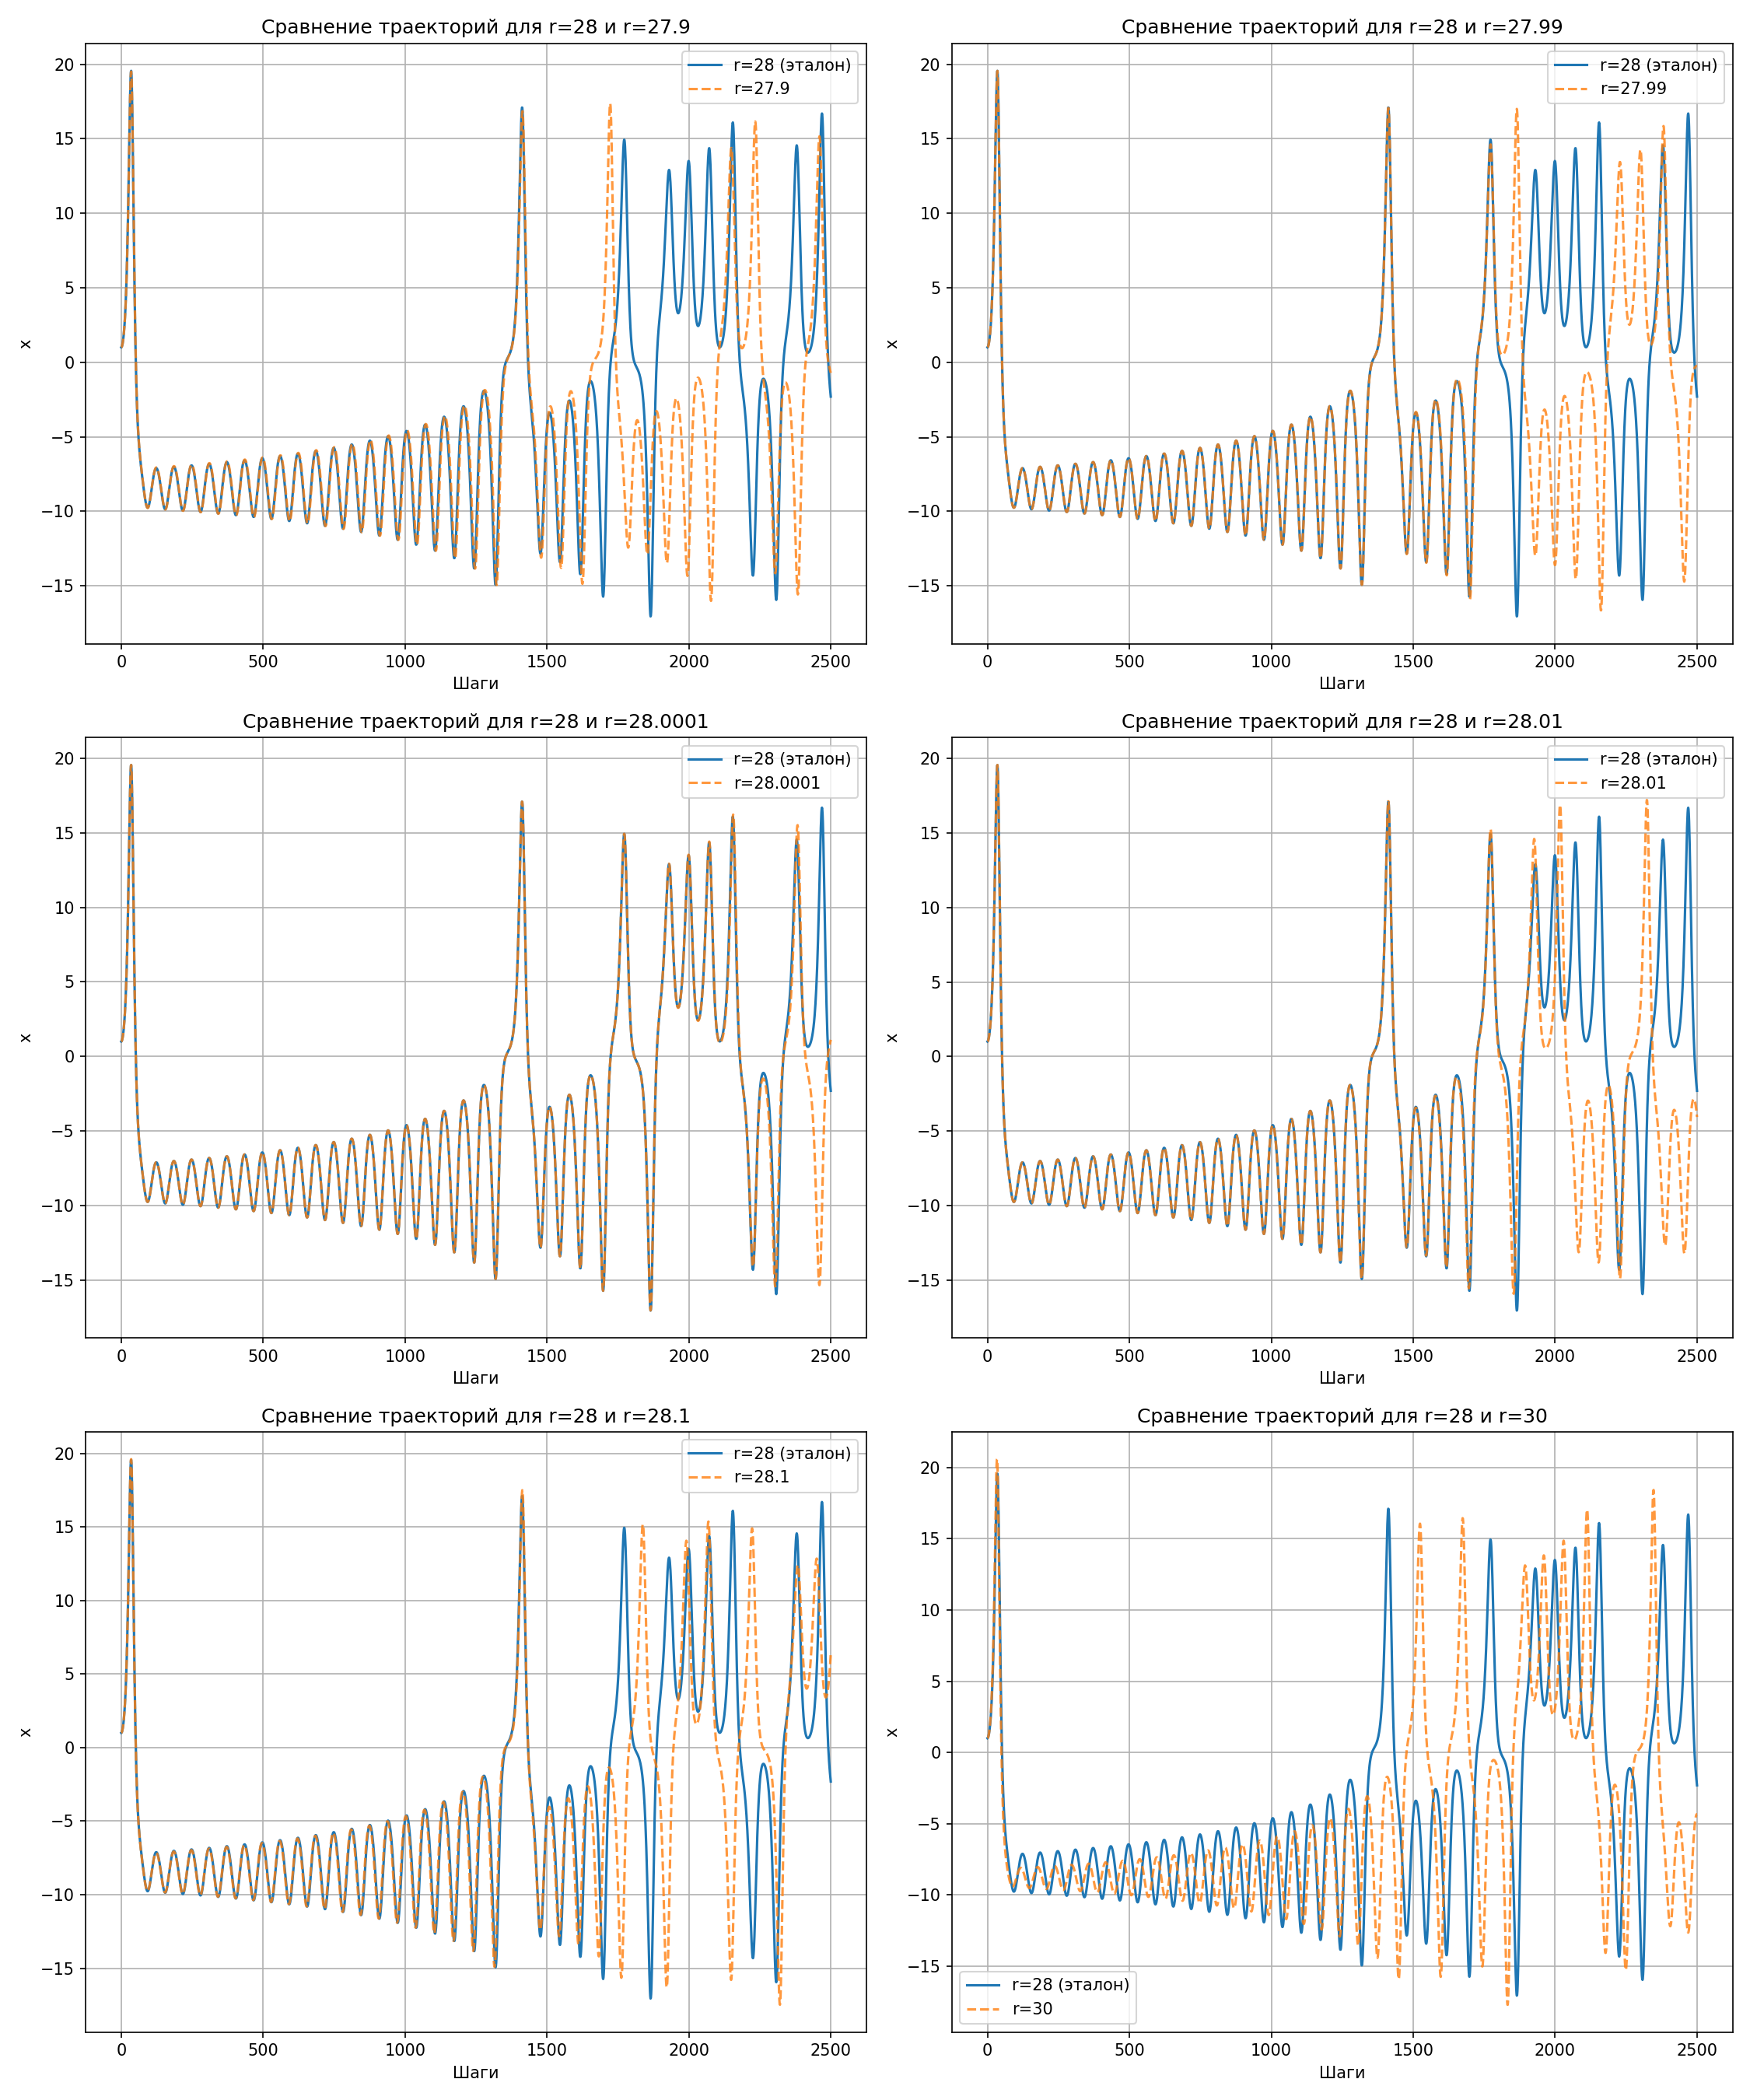
\includegraphics[width=\textwidth]{./dtw/rows.png}
        \caption{Построенные ряды Лоренца и их отличие от оригинального.}
        \label{fig:dtw_rows}
    \end{minipage}
\end{figure}

% <<< ИЗМЕНЕНИЕ: Заменяем mybox на conclusion
\begin{conclusion}
    Нельзя выделить строгую закономерность определения по dtw эффективности добавления
     рядов в выборку.r=28.0001 имеет наименьшее dtw,но  проигрывает в предсказании r=28.1.
\end{conclusion}

% ===================================================================
% ЧЕТВЕРТЫЙ ЭКСПЕРИМЕНТ
% ===================================================================
\newpage

\section{Эксперимент 4: Сравнение смещения центроидов кластеров}

\subsection{Описание эксперимента}
В данном эксперименте были скластеризованы:
\begin{itemize}
    \item 10000 точек базового ряда (получены \textbf{базовые} центроиды).
    \item Наборы из 10000 точек базового ряда и n точек добавленного
     ряда с разными $r$ (получены \textbf{смешанные} центроиды).
\end{itemize}
После этого к каждому базовому центроиду выбирался ближайший центроид 
из смешанных, и расстояние между ними усреднялось по всем парам.

\subsection{Результаты}

\begin{figure}[H]
    \centering
    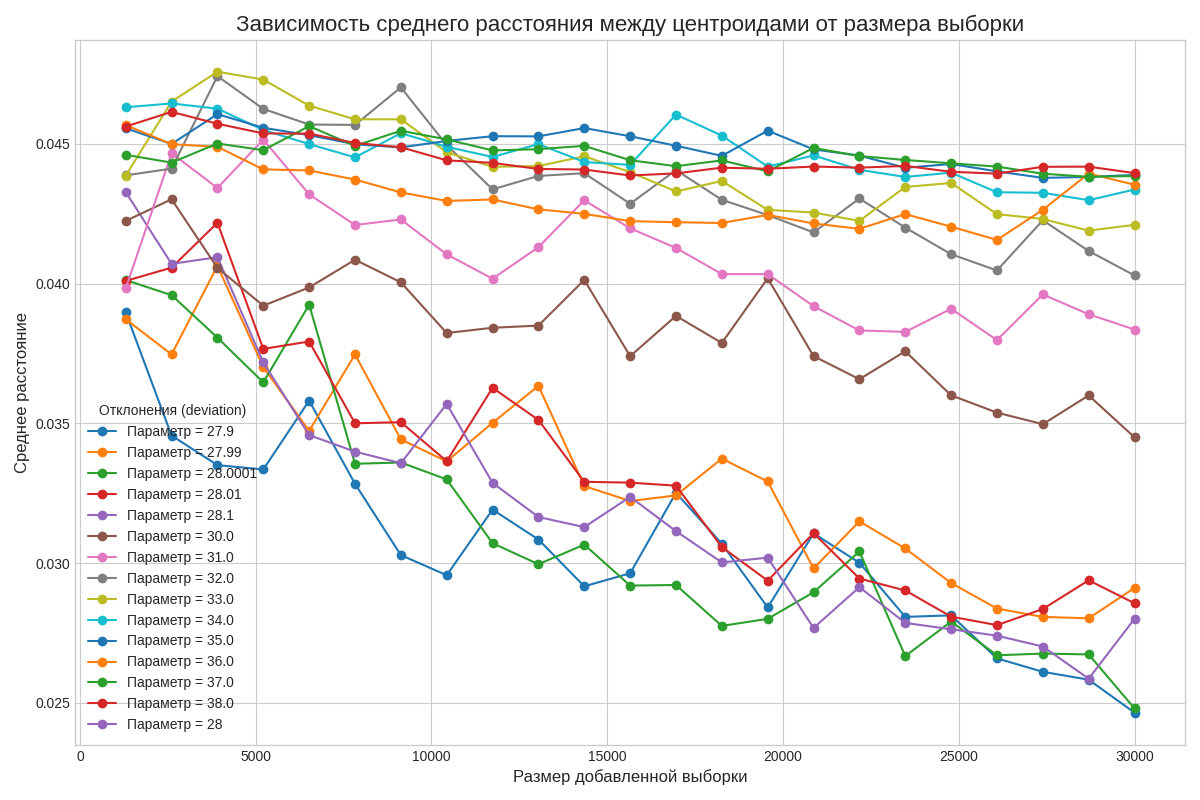
\includegraphics[width=\textwidth]{./centroids_diff/random_name.png}
    \caption{График зависимости  расстояний между центроидами.}
    \label{fig:centroids_diff}
\end{figure}

% <<< ИЗМЕНЕНИЕ: Заменяем mybox на conclusion
\begin{conclusion}
    У меня не получается обьяснить,почему при добавлении больших
     выборок второго ряда начинает снижаться разница между кластеризациями.
     При этом на далеких от исходного значениях параметра такого эффекта нет.
\end{conclusion}

% ===================================================================
% ПЯТЫЙ ЭКСПЕРИМЕНТ
% ===================================================================
\newpage

\section{Эксперимент 5: Сравнение метрик кластеризации при смешивании выборок}

\subsection{Описание эксперимента}
Данный эксперимент сравнивает метрики кластеризации при кластеризации на 
основе обучающей выборки, состоящей из `share * 10000` точек ряда с $\sigma=10,
 r=28, b=8/3$ и `(1-share) * 10000` точек ряда с другим значением $r$.

Были посчитаны следующие метрики:
\begin{itemize}
    \item WSS 
    \item $R^2$
    \item Calinski-Harabasz index
    \item Davies–Bouldin index
    \item Процент шума (noise\_percentage)
    \item Xie-Beni index
    \item Средний размер кластеров (avg\_cluster\_size)
\end{itemize}

\subsection{Результаты}
Были построены графики метрик для разных долей `share` примешанного ряда. 
\vspace{1cm} 
\begin{center}
    \href{https://disk.360.yandex.ru/d/lNCcbHohd4aaiA/%D0%A1%D1%80%D0%B0%D0%B2%D0%BD%D0%B5%D0%BD%D0%B8%D0%B5%20%D0%BC%D0%B5%D1%82%D1%80%D0%B8%D0%BA%20%D0%BA%D0%BB%D0%B0%D1%81%D1%82%D0%B5%D1%80%D0%B8%D0%B7%D0%B0%D1%86%D0%B8%D0%B8}{\textbf{ Яндекс диск с графиками}}
\end{center}
\vspace{1cm}

% <<< ИЗМЕНЕНИЕ: Заменяем mybox на conclusion
\begin{conclusion}
    На метриках ничего особенного интересного не заметил.
\end{conclusion}

% ===================================================================
% ШЕСТОЙ ЭКСПЕРИМЕНТ
% ===================================================================

\section{Эксперимент 6: Предсказание без использования исходного ряда}

\subsection{Описание эксперимента}
То же самое,что и в первом и седьмом эксперименте,но без обучающей выборки из оригинального ряда.
\begin{conclusion}
    С увеличением выборки уменьшается доля NP точек,но RMSE,MAPE падают не сильно.
\end{conclusion}
\subsection{Результаты}
\begin{figure}[H]
        \centering
        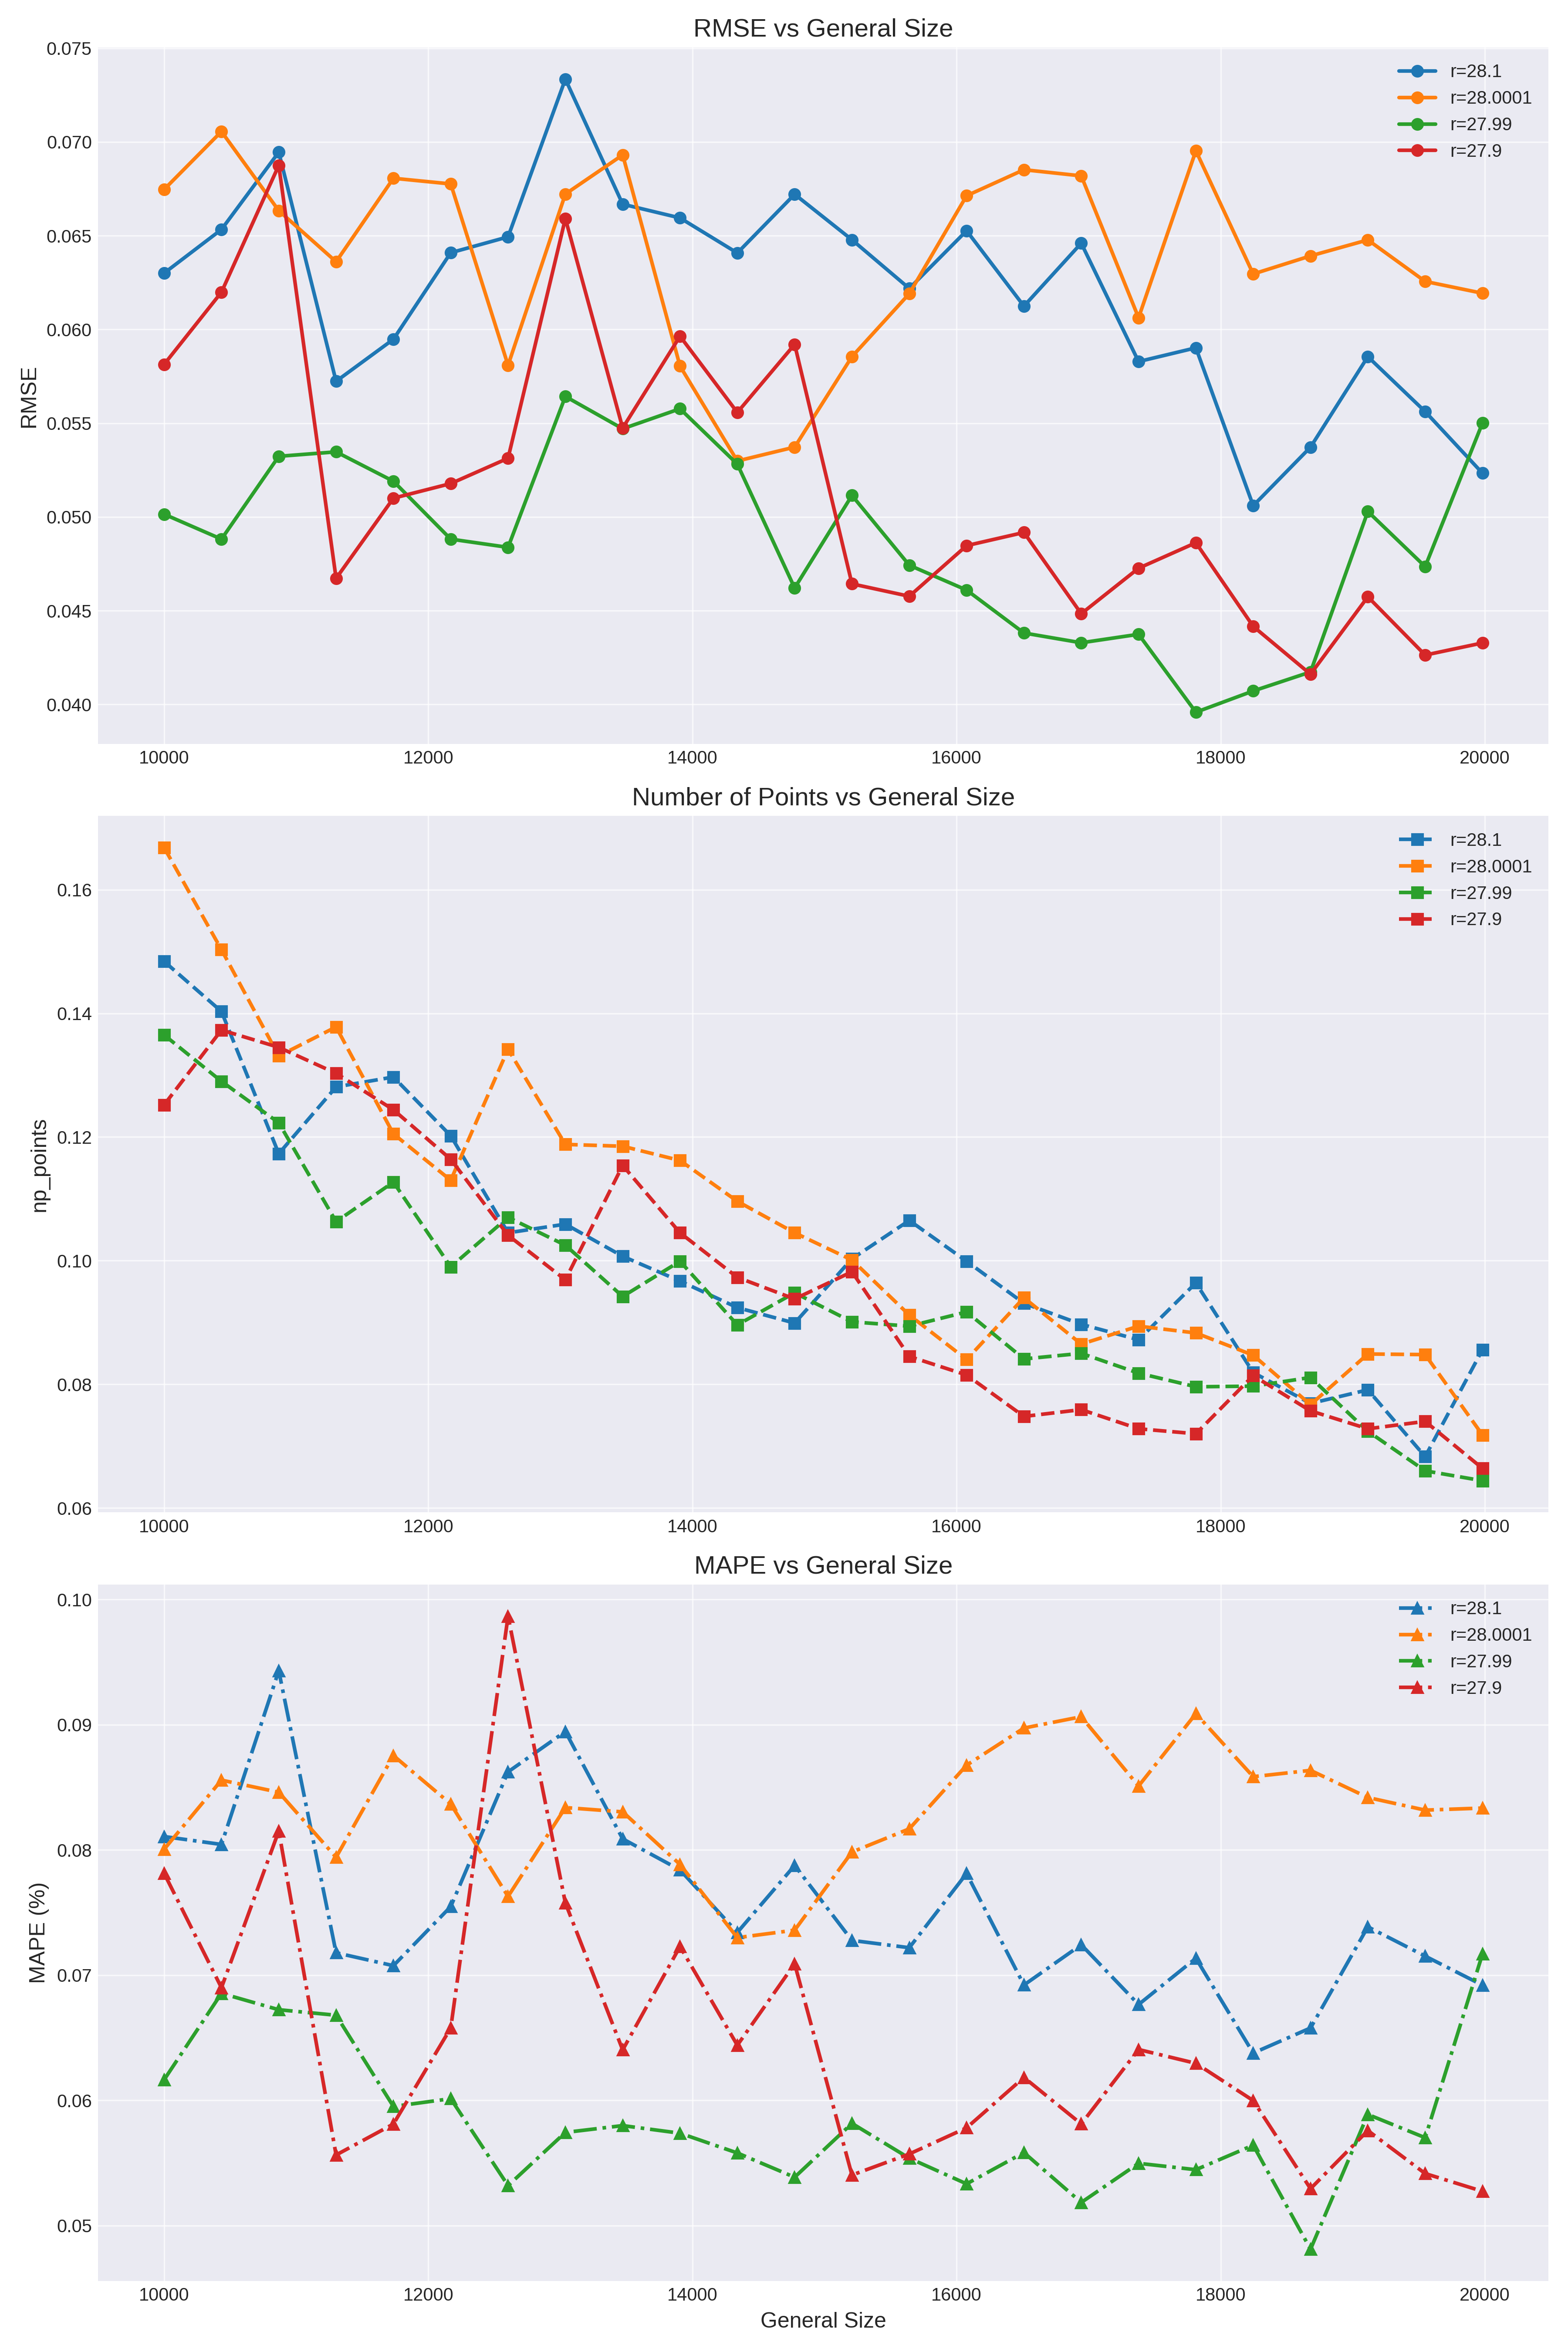
\includegraphics[width=\textwidth]{./Size_experiment/metrics_vs_general_size_best_experiments_2.png}
        \caption{Зависимость метрик от суммарного размера обучающей выборки добавленного ряда.}
        \label{fig:no_base_series}
\end{figure}

% <<< ИЗМЕНЕНИЕ: Заменяем mybox на conclusion


\newpage

\section{Эксперимент 7: Первый эксперимент без нормировки.}

\subsection{Описание эксперимента}
Данный эксперимент сравнивает 3 метрики при предсказании на 10 шагов вперед:
 RMSE, доля непрогнозируемых точек, MAPE для разных обучающих выборок.

Были посчитаны метрики для обучающей выборки, состоящей из 10000 точек ряда
 с $\sigma=10, r=28, b=8/3$, для которого мы предсказываем и переменным количеством 
 точек ряда с другим значением $r$. Были подсчитаны метрики для обучающей выборки 
 из переменного количества точек базового ряда с $\sigma=10, r=28, b=8/3$ (на графике обозначено как r=28).

На графике изображена зависимость метрик от суммарного размера обучающей выборки.

\subsection{Результаты}

\begin{figure}[H]
    \begin{minipage}[c]{0.3\textwidth} 
        В результате эксперимента получено, что для небольших отклонений 
        на разных участках может наблюдаться улучшение всех трех метрик, 
        сравнимое с добавлением выборки оригинального ряда. 
        \vspace{\baselineskip}
        
        Для добавленного ряда с $r=27.9$ и $r=27.99$ получаются результаты
         сравнимые по всем метрикам с выборкой только на основе базового ряда.
        \vspace{\baselineskip}

        При этом для $r=28.0001$ результаты получаются хуже чем для $r=28.1$.
         Все добавленные ряды уменьшают количество непрогнозируемых точек.
    \end{minipage}
    \hfill 
    \begin{minipage}[c]{0.68\textwidth} 
        \centering
        
\includegraphics[width=\textwidth]{./Size_experiment/metrics_vs_general_size_best_experiments.png}
        \caption{Зависимость метрик от суммарного размера обучающей выборки.}
        \label{fig:best_exp_original} % Изменена метка во избежание дублирования
    \end{minipage}
\end{figure}

\begin{figure}[H]
    \begin{minipage}[c]{0.3\textwidth} 
        В файле \texttt{unlucky\_experiments.png} можно увидеть менее удачные 
        расширения обучающих выборок за счет добавления выборок с рядами с параметрами 
        $r=28.01$, $r=30$, $r=38$, $r=27$, поскольку они не дают выигрыш по всем 
        трем метрикам, но могут дать выигрыш по количеству непрогнозируемых точек или метрикам качества предсказания.
    \end{minipage}
    \hfill
    \begin{minipage}[c]{0.68\textwidth}
        \centering
        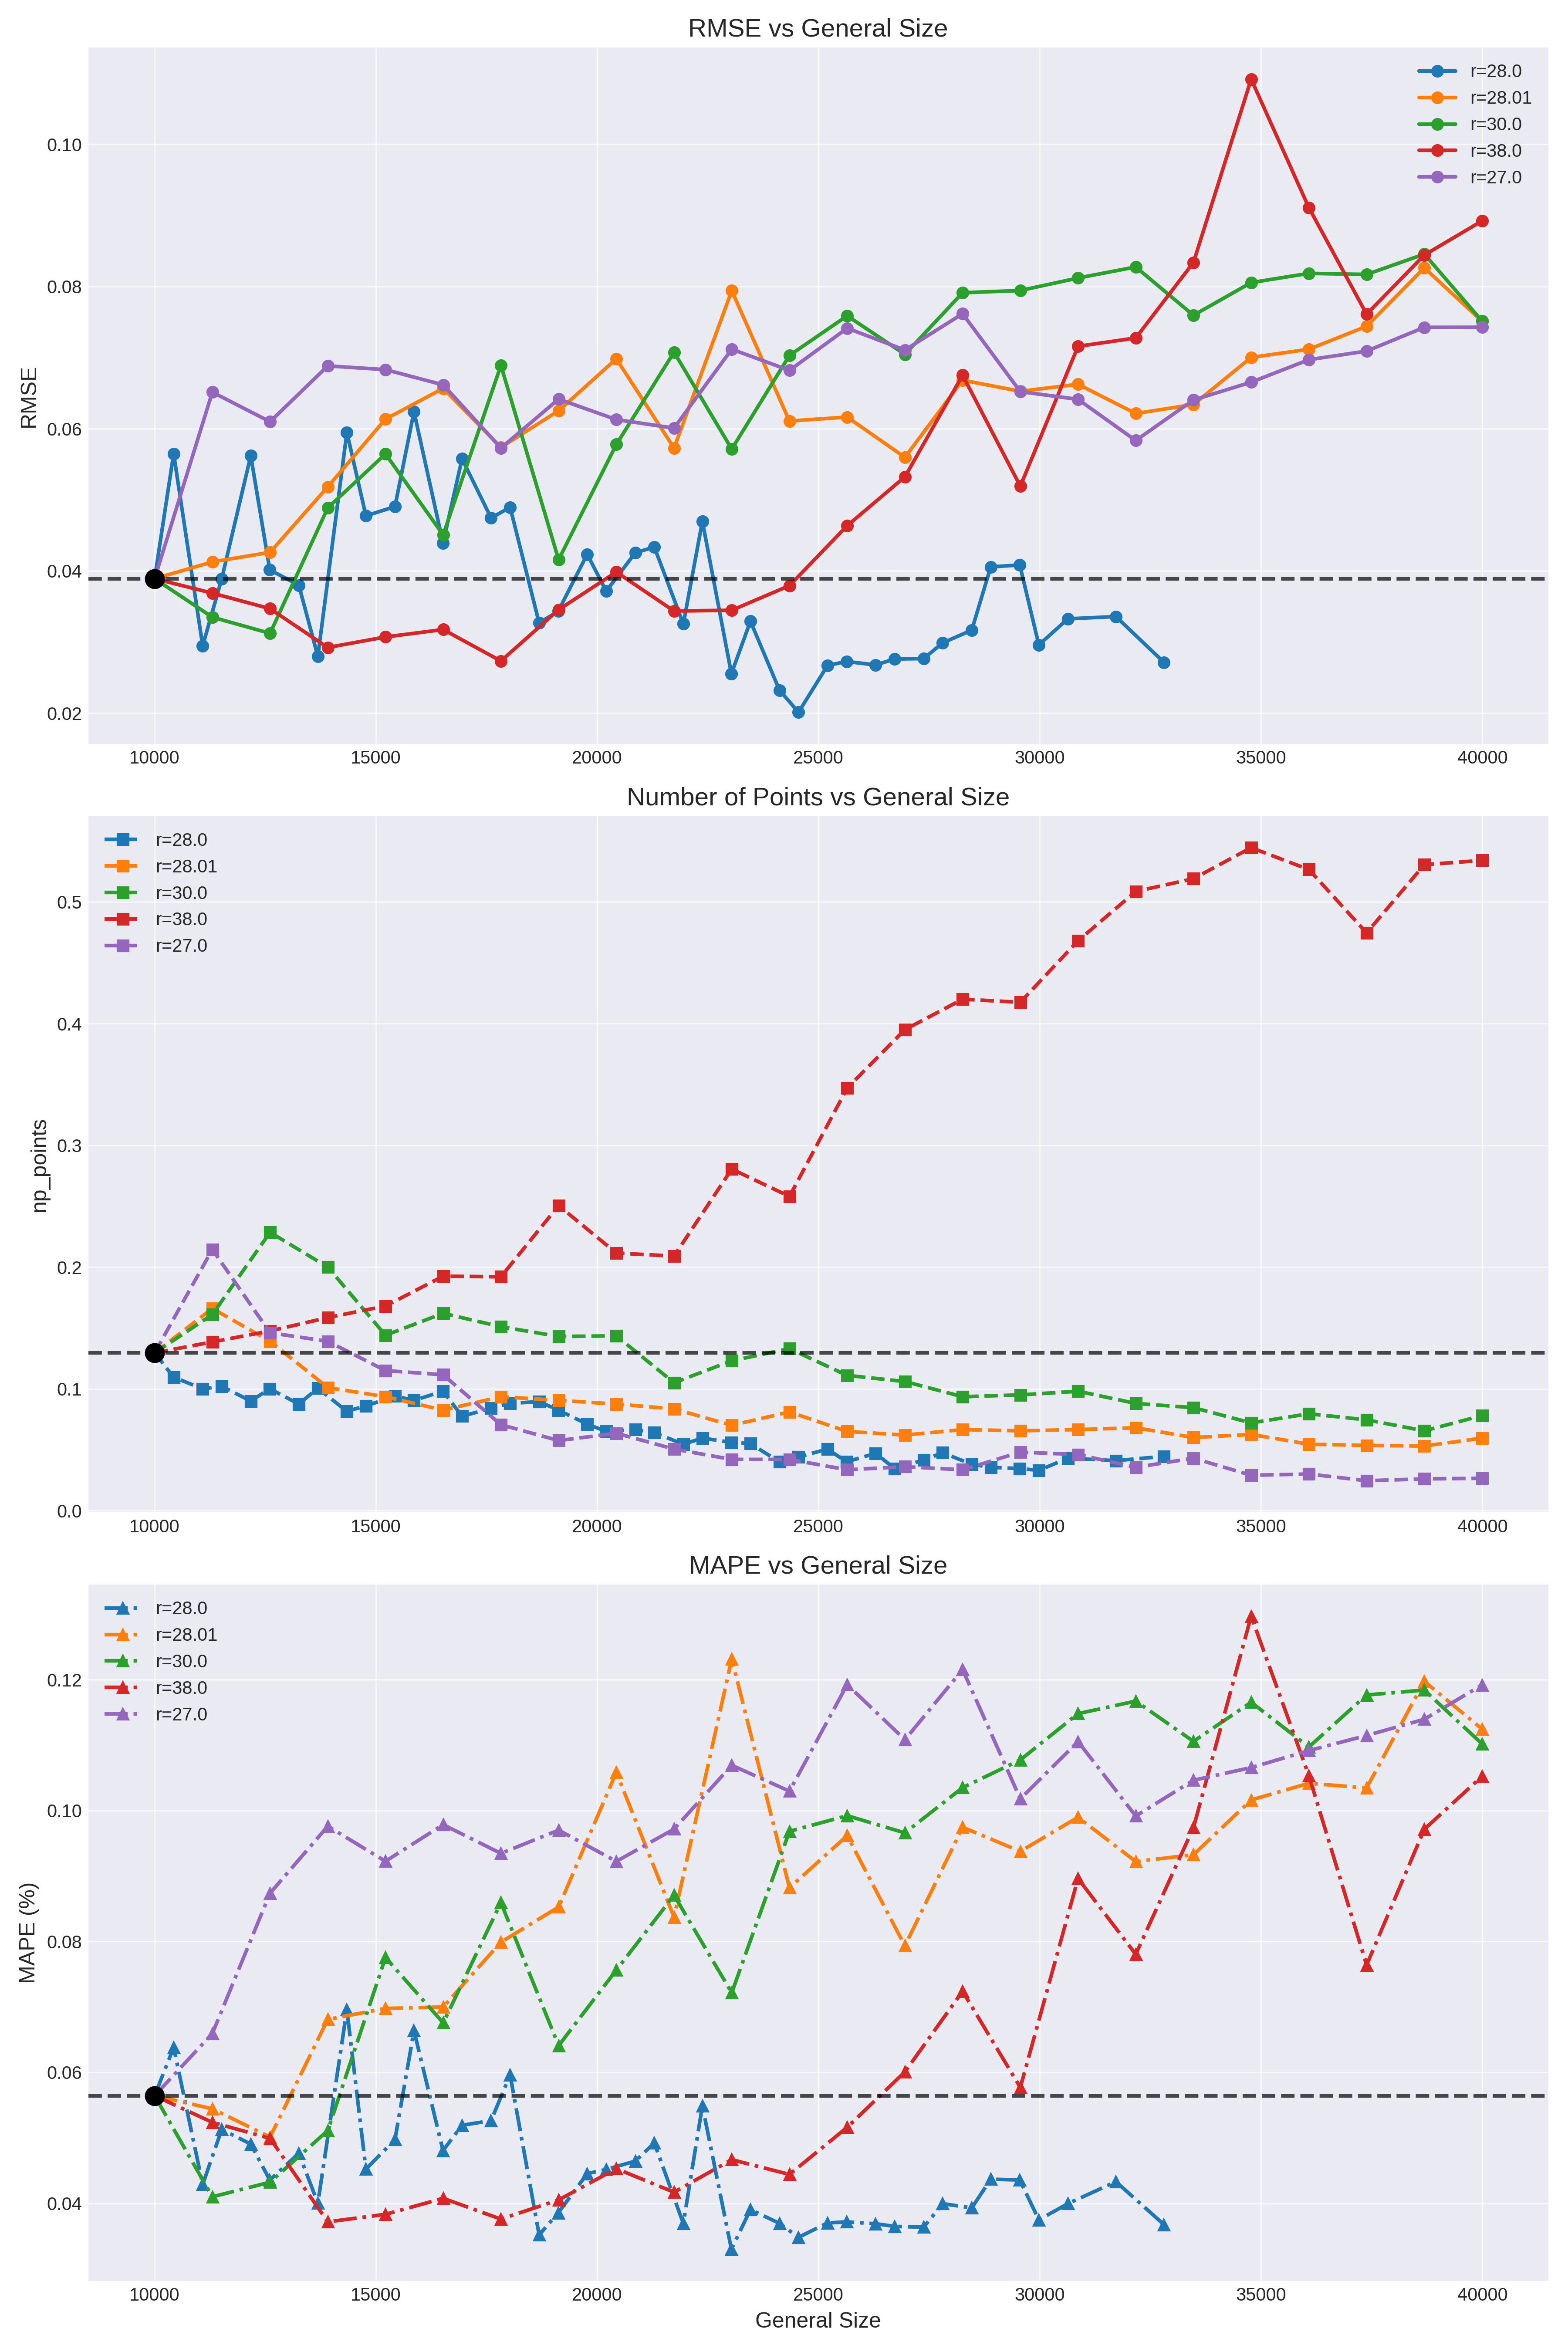
\includegraphics[width=\textwidth]{./Size_experiment/unlucky_experiments.png}
        \caption{Менее удачные расширения обучающих выборок.}
        \label{fig:unlucky_exp_original} % Изменена метка во избежание дублирования
    \end{minipage}
\end{figure}


\begin{conclusion}
    Для добавленного ряда с $r=27.9$ и $r=27.99$ получаются результаты 
    сравнимые по всем метрикам с выборкой только на основе базового ряда.
    
    Менее удачные расширения обучающих выборок (с $r=28.01, r=30, r=38, r=27$)
     не дают выигрыш по всем трем метрикам, но могут дать выигрыш по количеству
      непрогнозируемых точек или метрикам качества предсказания.
    
    Почему предсказание с $r=28.0001$ хуже чем с $r=28.1$ меня вгоняет в тупик.
\end{conclusion}

% ===================================================================
% КОНЕЦ БЛОКА ДЛЯ СЕДЬМОГО ЭКСПЕРИМЕНТА
% ===================================================================
\newpage
\begin{conclusion}
    По итогу,непонятно,что стоит исследовать дальше.стоит ли продолжать исследовать
     близкие к ряду Лоренца значения параметров или лучше исследовать другие хаотичсекие временные ряды вроде Хенона/Ресслера,
     или может быть стоит поэксперементировать над реальными данными.
\end{conclusion}
\end{document}